\chapter{\texorpdfstring{EPC Analysis}{EPC Analysis}}
\label{ch:16a}
\lecturemeta{Lezione 16a \quad\textbullet\quad 2026-07-04 \quad\textbullet\quad Roberto Bruni}{Weske, \emph{Business Process Management}, Ch.6}

Con le lezioni precedenti abbiamo costruito una teoria completa per i Petri net: sappiamo verificare boundedness, liveness e — per i workflow net — la \hyperref[ch:12]{soundness}. Ora chiudiamo il cerchio tornando alle notazioni di alto livello: gli \textbf{EPC} (Event-driven Process Chain), introdotti in \hyperref[ch:07a]{07a — EPC e BPMN}. Il problema è che gli EPC sono nati come linguaggio \textbf{informale}, pensato per la comunicazione fra persone: sono semplici e piacciono, ma \textbf{non hanno una semantica formale univoca}. Diagrammi ambigui o addirittura scorretti possono nascere già in fase di design.

L'idea di questa lezione è dare agli EPC una semantica precisa \textbf{traducendoli in workflow net}, così da poter riusare tutti gli strumenti di verifica:

\begin{boxabstract}{La strategia in una frase}
Traduciamo l'EPC in un workflow net $N$; diciamo che \textbf{l'EPC è sound se il suo net $N$ è sound}. La soundness del net la sappiamo già verificare (liveness + boundedness di $N^\star$, anche con tool come WoPeD). \textbf{Attenzione:} \emph{non} esiste un unico modo di tradurre — vedremo tre approcci diversi, con pregi e difetti differenti.
\end{boxabstract}

\begin{figure}[!htb]
\centering

\includegraphics[width=0.74\linewidth,height=0.34\textheight,keepaspectratio]{images/16a-epc-analysis_p2_object-example.png}
\caption{Un tipico EPC: eventi (esagoni), functions (rettangoli), connettori $\wedge$ (AND), $\vee$ (OR), XOR. Vogliamo capire se un processo così è "corretto" — e per farlo lo trasformiamo in un Petri net.}
\end{figure}

\section{\texorpdfstring{Gli ingredienti di un EPC e la loro traduzione}{Gli ingredienti di un EPC e la loro traduzione}}

Un EPC è fatto di pochi elementi. Il punto di partenza della traduzione è una corrispondenza naturale con i pezzi di un Petri net.

\begin{boxdefinition}{Corrispondenza EPC $\leftrightarrow$ net (commonalities)}
\begingroup\small
\begin{tabularx}{\linewidth}{>{\raggedright\arraybackslash}X>{\raggedright\arraybackslash}X}
\toprule
\textbf{Elemento EPC} & \textbf{Frammento di net} \\
\midrule
\textbf{event} (esagono) & \textbf{place} \\
\textbf{function} (rettangolo) & \textbf{transition} \\
\textbf{control flow} (arco tratteggiato) & \textbf{arco} \\
\textbf{connector} ($\wedge$, $\vee$, XOR) & piccolo \textbf{frammento} di net (vedi sotto) \\
\bottomrule
\end{tabularx}
\endgroup

L'intuizione è coerente con la semantica dei net: un event è uno \emph{stato} del processo (come un place che "contiene" o meno un token), una function è un \emph{task} che avviene (come una transition che scatta).
\end{boxdefinition}

La traduzione vera e propria segue \textbf{tre step}.

\begin{figure}[!htb]
\centering
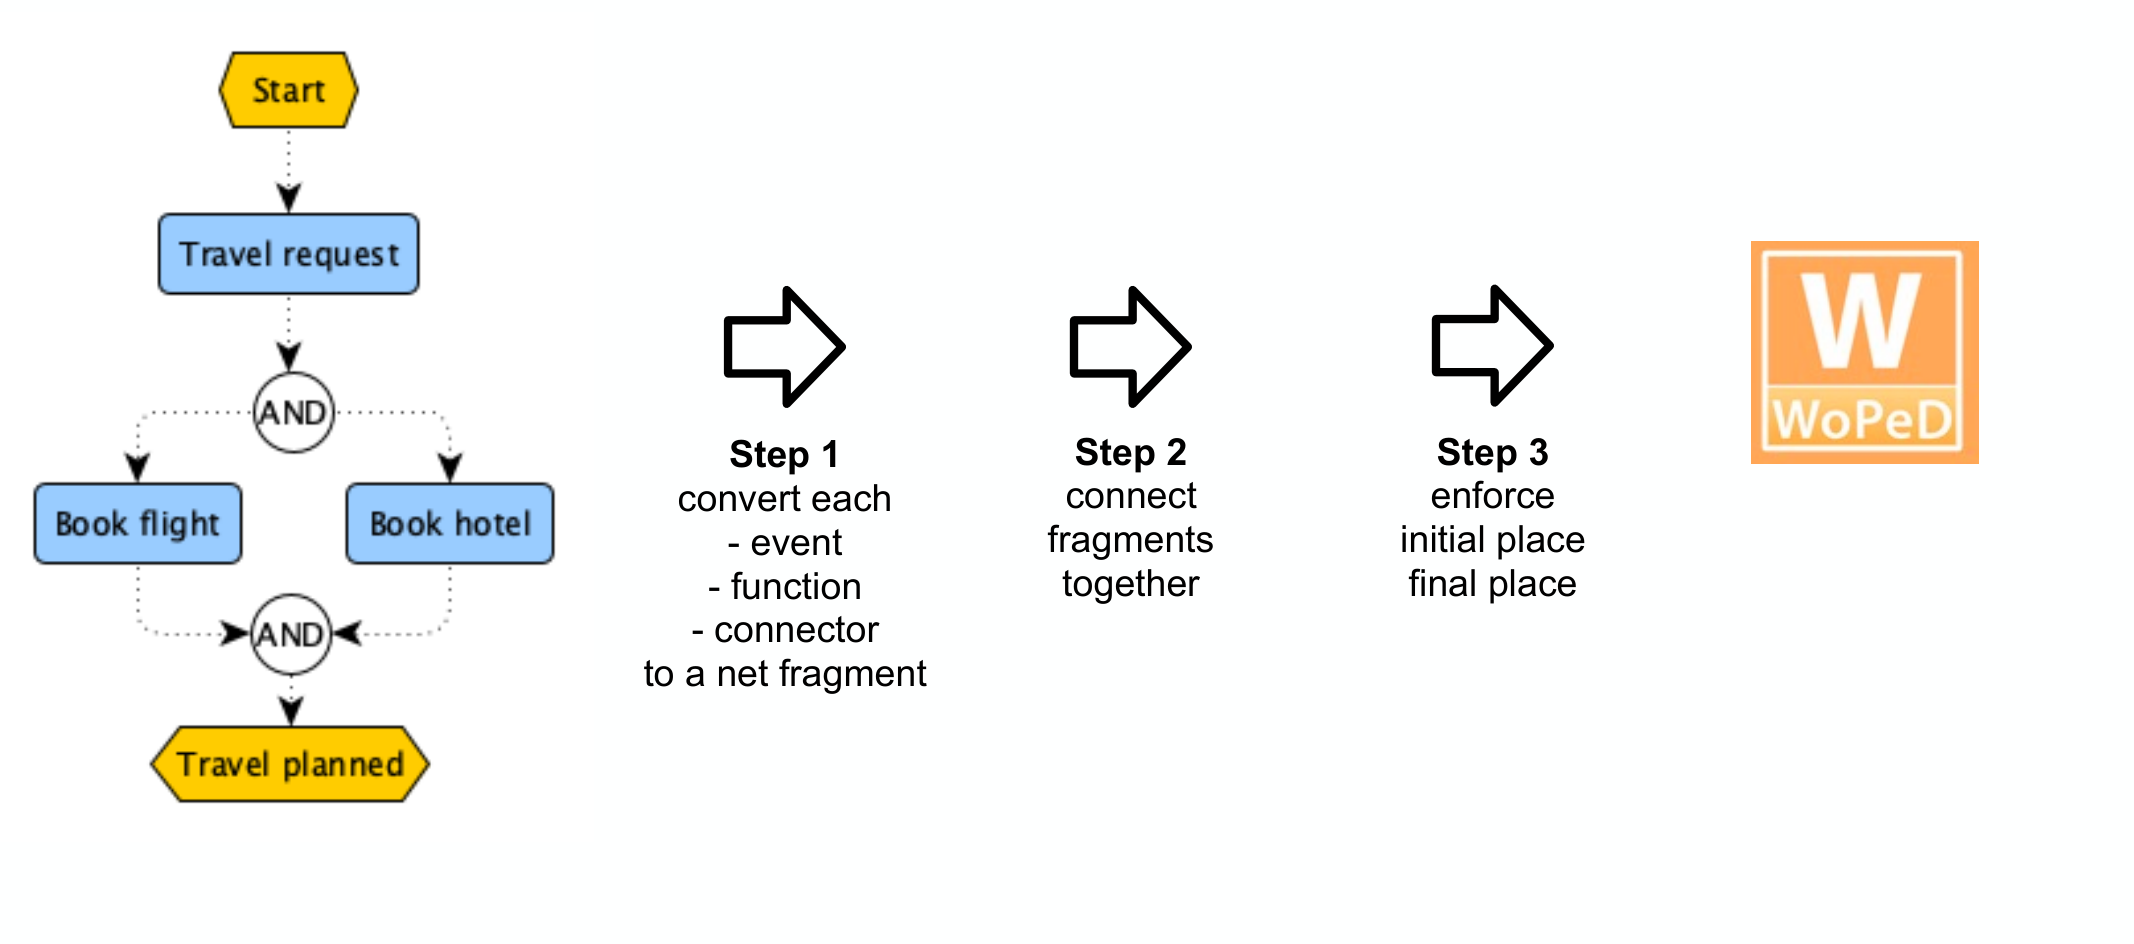
\includegraphics[width=0.74\linewidth,height=0.34\textheight,keepaspectratio]{images/16a-epc-analysis_p9_three-steps.png}
\caption{Da EPC a wf net in tre step, verificabili poi con un tool come WoPeD.}
\end{figure}

\begin{boxnote}{I tre step della traduzione}
\begin{enumerate}
\item \textbf{Step 1 — frammenti locali}: si sostituisce \emph{separatamente} ogni event, function e connector con un piccolo frammento di net.
\item \textbf{Step 2 — connessione dei frammenti}: si "cuciono" insieme i frammenti. Due stili possibili (vedi sotto): \emph{dummy style} o \emph{fusion style}.
\item \textbf{Step 3 — unico inizio / unica fine}: un workflow net richiede \textbf{un solo} place iniziale $i$ e \textbf{un solo} place finale $o$. Se l'EPC ha più eventi start (o più eventi end), li si unifica con un connettore (tipicamente XOR per lo start; XOR/AND/OR per l'end a seconda del significato voluto).
\end{enumerate}
\end{boxnote}

\subsection{\texorpdfstring{Step 2: dummy style vs fusion style}{Step 2: dummy style vs fusion style}}

Quando si collegano due frammenti, il primo produce un place-di-uscita e il secondo si aspetta un place-di-ingresso: mettendoli insieme rischiamo di avere \emph{due place consecutivi} (o due transition consecutive), che nei Petri net non è ammesso (place e transition devono alternarsi).

\begin{itemize}
\item \textbf{Dummy style}: si inserisce un elemento "fittizio" di raccordo — una \textbf{dummy transition} fra due place, o un \textbf{dummy place} fra due transition — per ripristinare l'alternanza.
\item \textbf{Fusion style}: si \textbf{fondono} i due place (o le due transition) adiacenti in un unico nodo. Più compatto, ma va fatto con attenzione.
\end{itemize}

\subsection{\texorpdfstring{Step 1: i frammenti dei connettori}{Step 1: i frammenti dei connettori}}

I connettori sono la parte delicata. AND e XOR hanno traduzioni "pulite"; l'OR è il problema centrale di tutta la lezione.

\begin{boxdefinition}{Frammenti dei connettori (traduzione base)}
\begin{itemize}
\item \textbf{AND split} ($\wedge$): un place che entra in una \textbf{transition}, che a sua volta mette un token in \emph{tutti} gli output place $\rightarrow$ esegue \textbf{tutti} i rami in parallelo.
\item \textbf{AND join} ($\wedge$): una transition che richiede un token da \emph{tutti} gli input place $\rightarrow$ \textbf{sincronizza} i rami.
\item \textbf{XOR split}: un place che alimenta \textbf{più transition} in conflitto $\rightarrow$ se ne sceglie \textbf{una sola} (scelta esclusiva).
\item \textbf{XOR join}: \textbf{più transition} che confluiscono in un unico place $\rightarrow$ il flusso prosegue non appena arriva \textbf{uno} dei rami.
\item \textbf{OR split} ($\vee$): "\textbf{xor + and}" $\rightarrow$ può attivare \textbf{uno, alcuni o tutti} i rami. Si realizza combinando una scelta XOR con una diramazione AND (vedi figura).
\item \textbf{OR join} ($\vee$): dovrebbe attendere e sincronizzare \textbf{solo i rami che sono stati effettivamente attivati} — ed è qui che nascono le ambiguità.
\end{itemize}
\end{boxdefinition}

\begin{figure}[!htb]
\centering
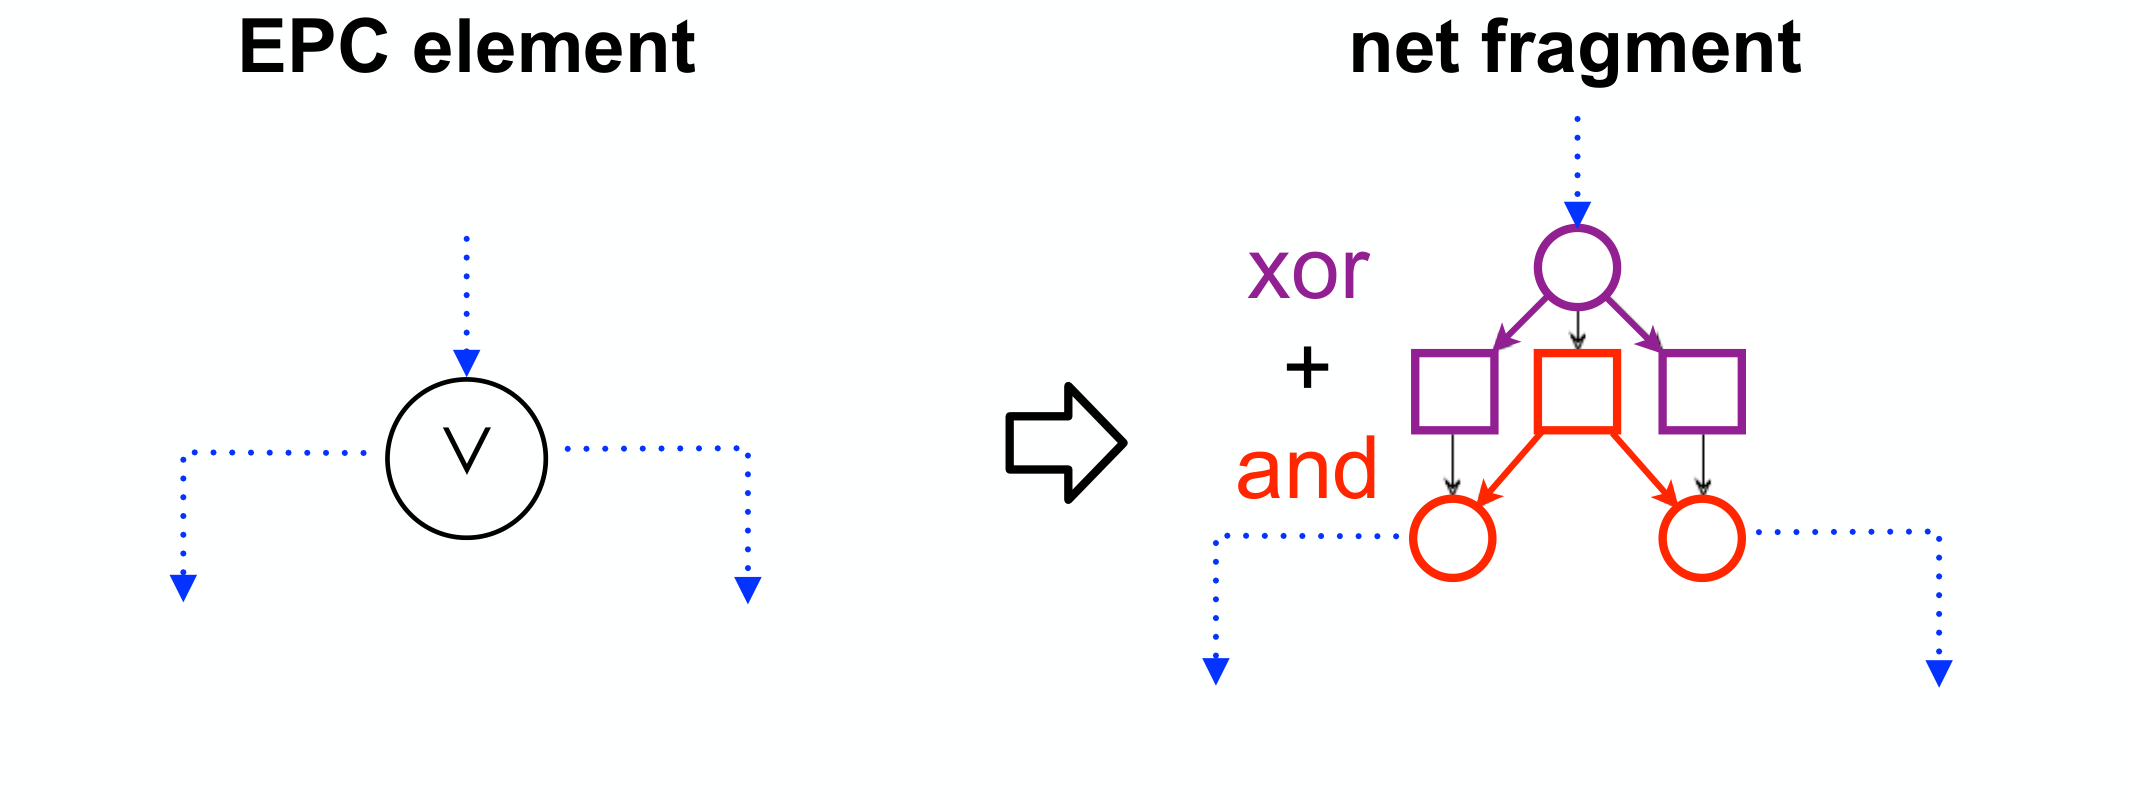
\includegraphics[width=0.74\linewidth,height=0.34\textheight,keepaspectratio]{images/16a-epc-analysis_p23_or-split.png}
\caption{L'\textbf{OR split} ($\vee$) come "xor + and": lo strato XOR sceglie \emph{quale sottoinsieme} di rami attivare, lo strato AND li lancia. Così si coprono tutti i casi "uno, alcuni o tutti".}
\end{figure}

\begin{figure}[!htb]
\centering
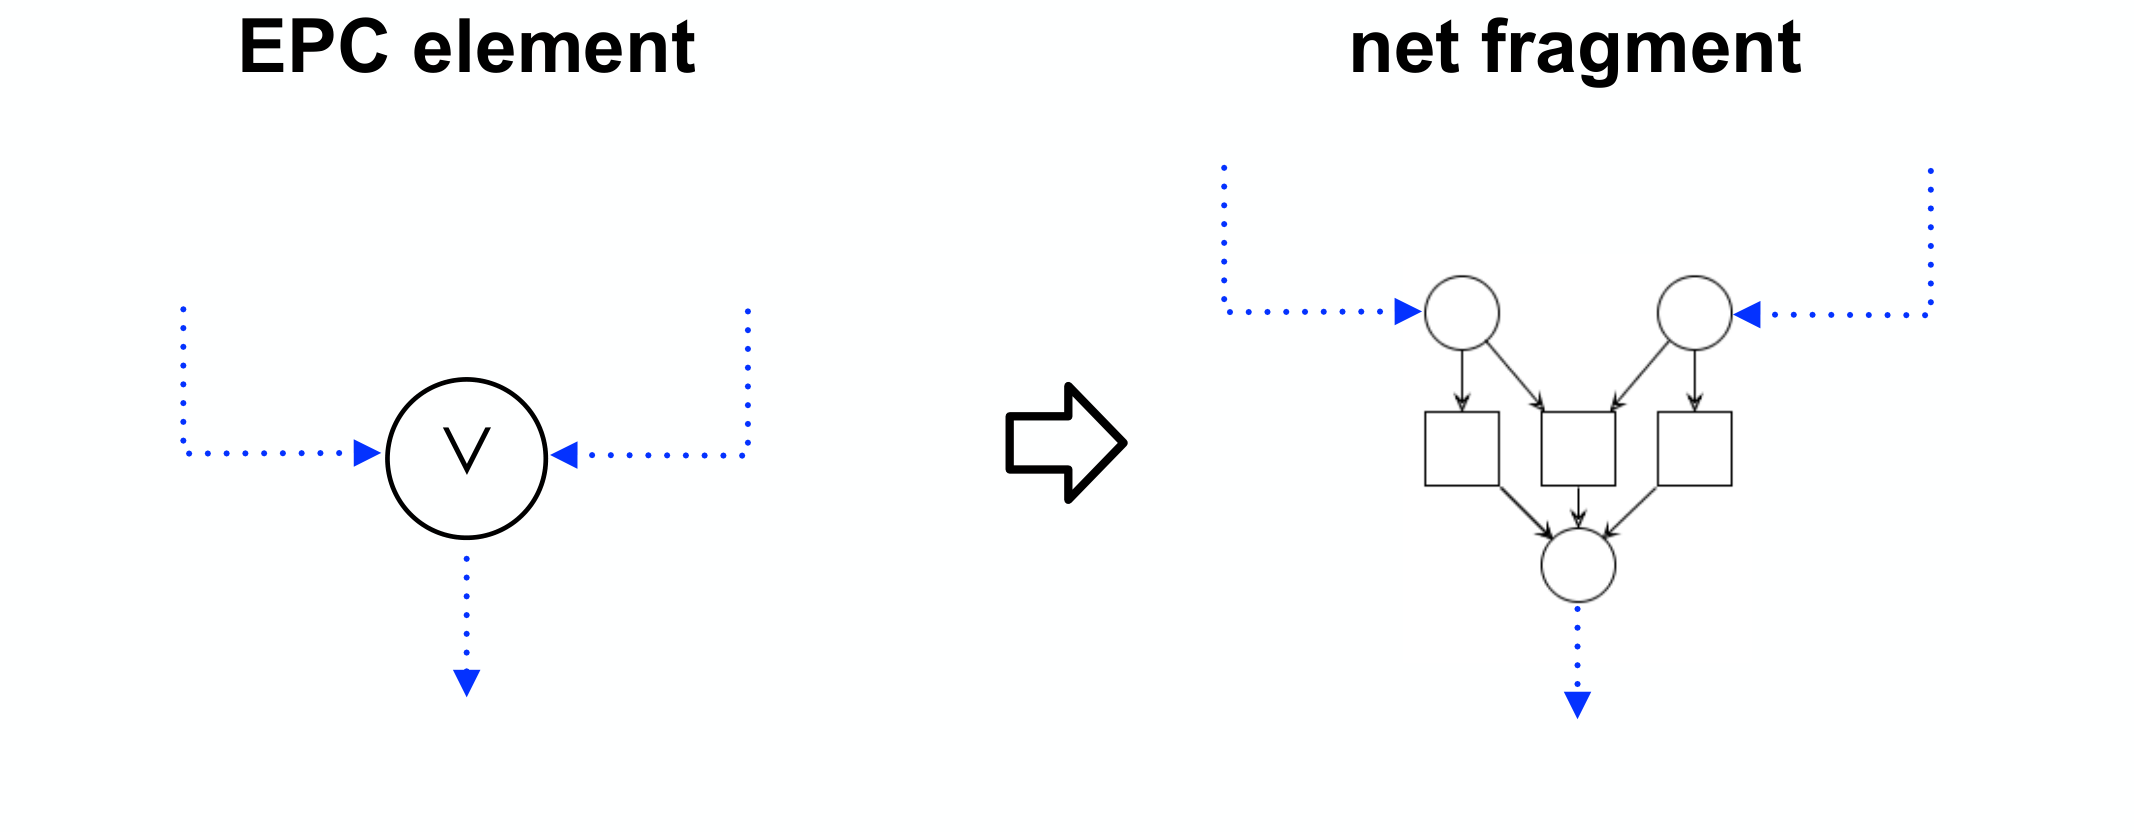
\includegraphics[width=0.74\linewidth,height=0.34\textheight,keepaspectratio]{images/16a-epc-analysis_p24_or-join.png}
\caption{L'\textbf{OR join} ($\vee$): dovrebbe sincronizzare \emph{solo} i rami attivati. Ma il frammento "non sa" quanti rami sono stati attivati dallo split corrispondente — da qui l'ambiguità semantica che rende difficile l'analisi.}
\end{figure}

\section{\texorpdfstring{Tre approcci alla traduzione}{Tre approcci alla traduzione}}

Il cuore della lezione è che \textbf{non c'è una traduzione unica}: si presentano tre approcci, con un compromesso diverso fra facilità, applicabilità e qualità del risultato.

\begin{boxabstract}{I tre approcci a confronto}
\begingroup\small
\begin{tabularx}{\linewidth}{>{\raggedright\arraybackslash}X>{\raggedright\arraybackslash}X>{\raggedright\arraybackslash}X>{\raggedright\arraybackslash}X>{\raggedright\arraybackslash}X}
\toprule
\textbf{} & \textbf{Difficoltà} & \textbf{Stile} & \textbf{Applicabilità} & \textbf{Risultato} \\
\midrule
\textbf{1°} & facile & fusion & \textbf{qualsiasi} EPC & probabilmente \textbf{unsound} $\rightarrow$ si ripiega su \emph{relaxed soundness} \\
\textbf{2°} & media (dipende dal contesto) & dummy & EPC \textbf{semplificato}: alternanza event/function, \textbf{niente OR} & \textbf{free-choice net} \\
\textbf{3°} & difficile (dipende dal contesto) & dummy & EPC \textbf{decorato}: join-split corrispondenti, policy per gli OR & \textbf{analisi accurata} \\
\bottomrule
\end{tabularx}
\endgroup

In breve: o accetti \emph{qualsiasi} diagramma ma ottieni poca garanzia; o restringi la sintassi (via gli OR) e ottieni una bella classe di net; o chiedi all'utente di \emph{decorare} il diagramma e ottieni l'analisi migliore.
\end{boxabstract}

\section{\texorpdfstring{Primo approccio: traduzione diretta (e la relaxed soundness)}{Primo approccio: traduzione diretta (e la relaxed soundness)}}

Il primo approccio traduce \textbf{qualsiasi} EPC alla lettera, in fusion style. Il vantaggio è la generalità; lo svantaggio è che il net risultante è \textbf{quasi sempre non sound}, soprattutto per colpa degli OR.

Il razionale (Dehnert \& Rittgen, 2001) è pragmatico: l'EPC va usato \emph{fin dalle prime fasi} del design, quando il modello è ancora impreciso. Serve allora una rappresentazione formale che \textbf{preservi le ambiguità} invece di nasconderle, così da poter scovare i difetti presto.

\begin{figure}[!htb]
\centering
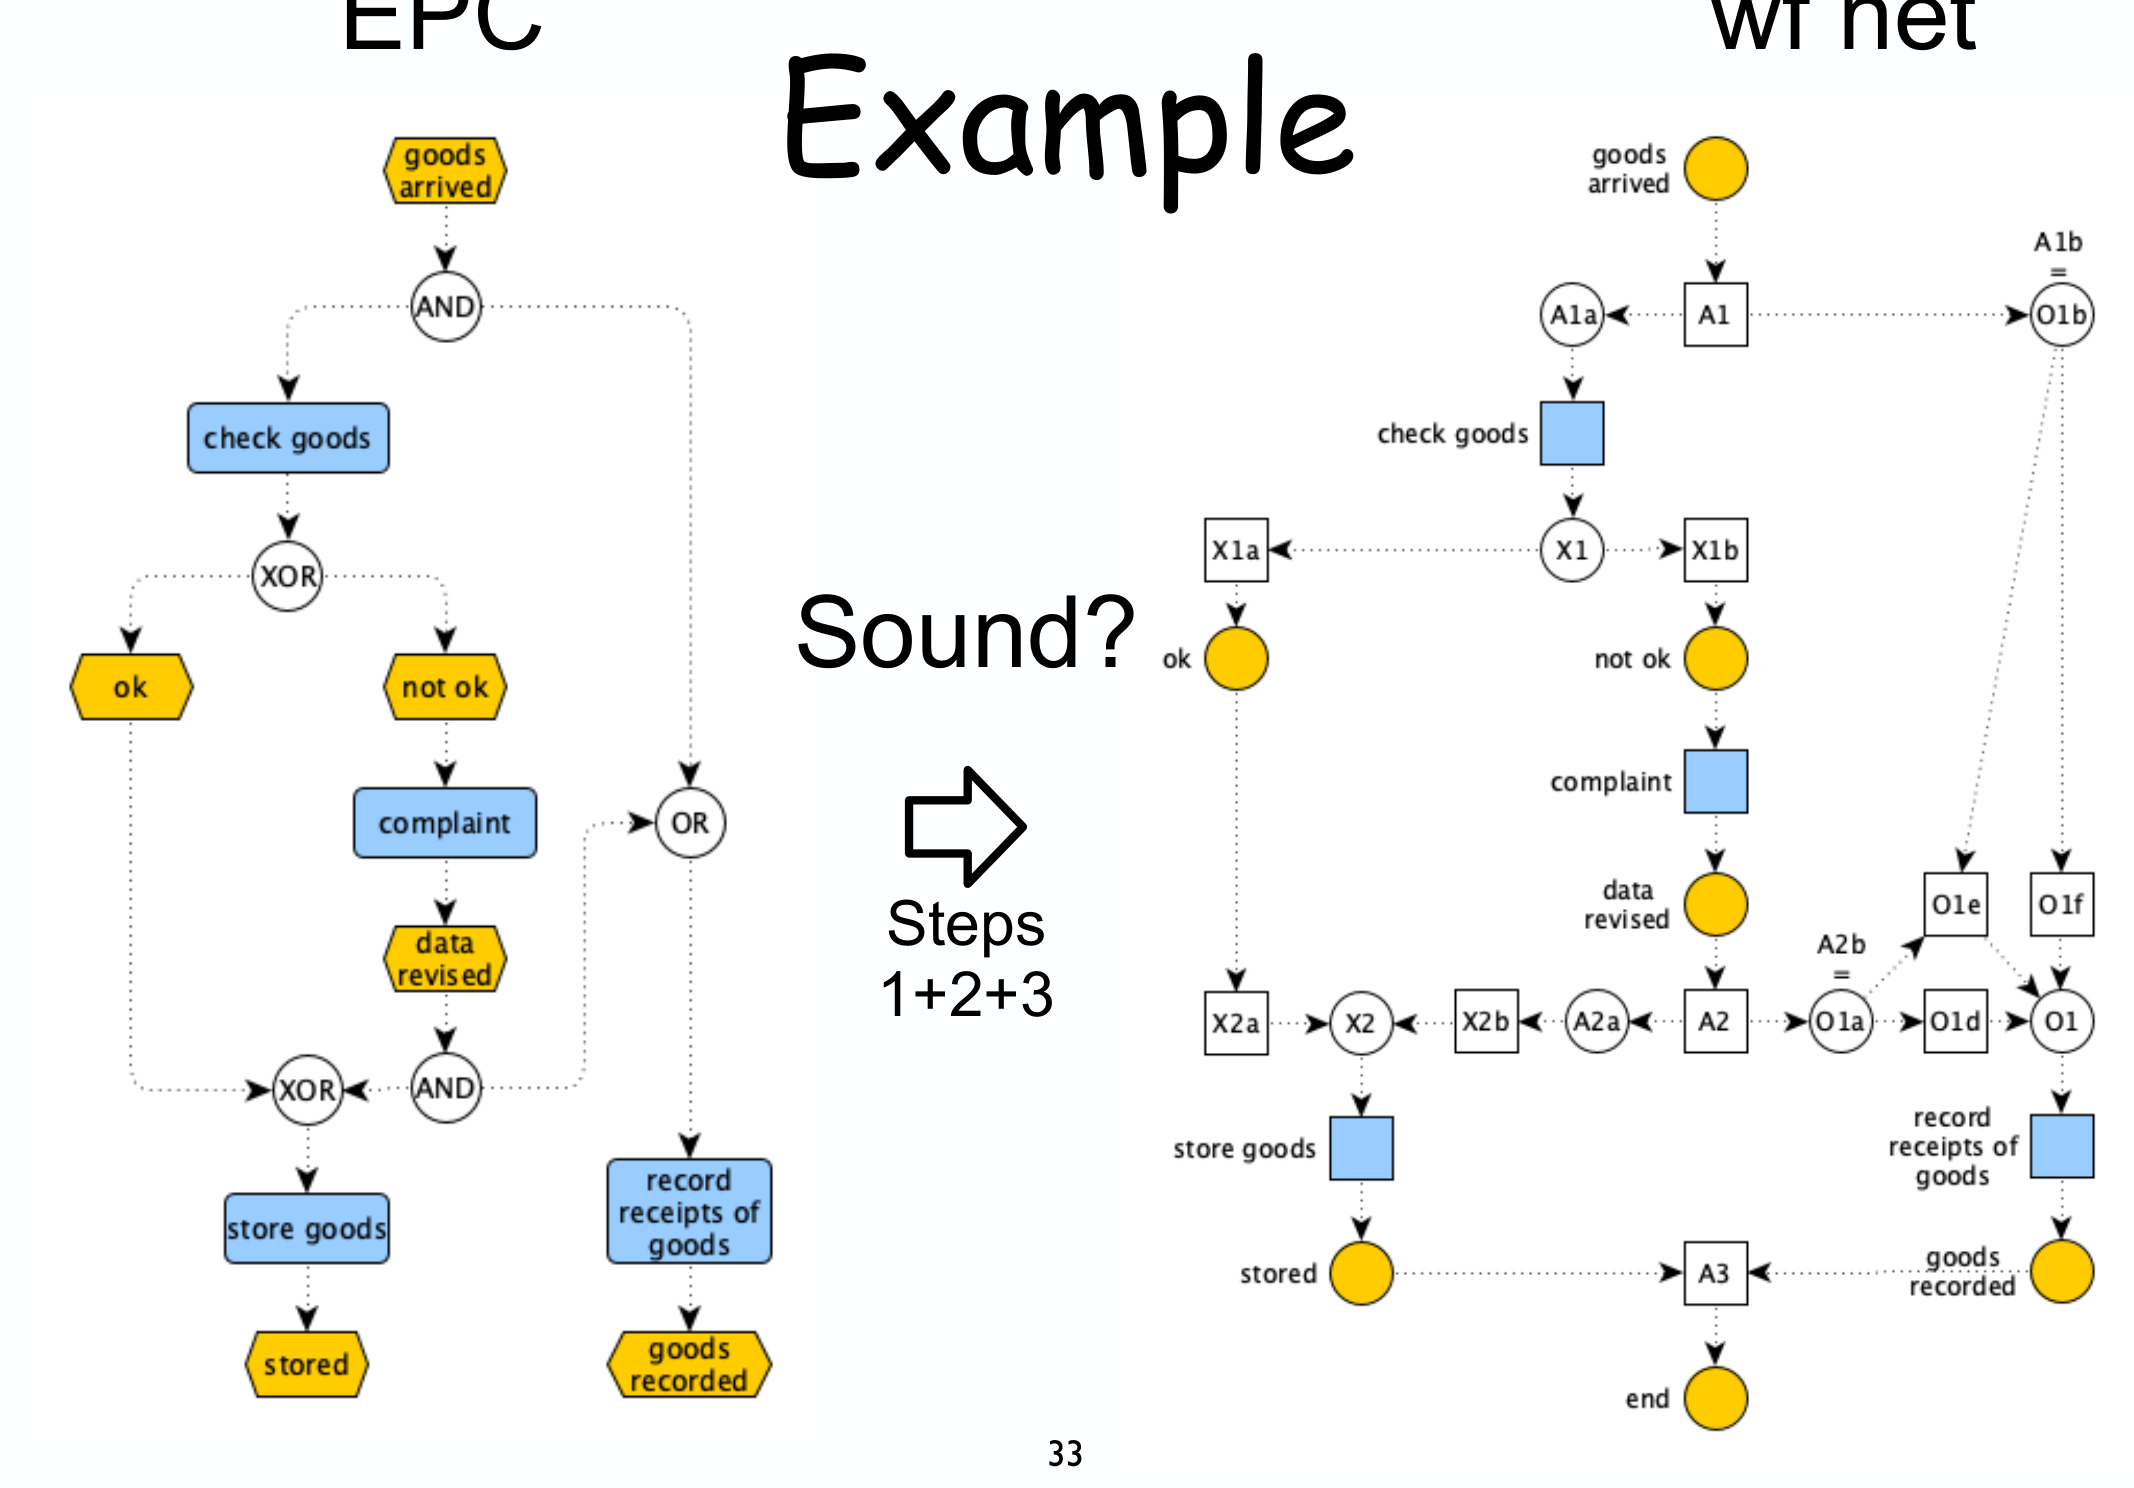
\includegraphics[width=0.74\linewidth,height=0.34\textheight,keepaspectratio]{images/16a-epc-analysis_p33_example-epc-wfnet.png}
\caption{L'esempio guida: EPC (sinistra) e la sua traduzione in wf net (destra) dopo gli step 1+2+3. La domanda è "\textbf{Sound?}". La risposta, ahimè, è \textbf{no}.}
\end{figure}

Perché non è sound? Il colpevole è l'\textbf{OR join}. Semanticamente vorremmo che, arrivato un token da un ramo, la join "capisca" se aspettarne un altro. Ma il net non ha questa informazione:

\begin{boxwarning}{Il difetto dell'OR join}
\begin{itemize}
\item Quando arriva un token, "la cosa giusta da fare" sarebbe scattare \emph{una} certa transition… ma \textbf{anche altre transition risultano abilitate} (è la semantica dell'OR!).
\item Il risultato: la \textbf{proper completion non è garantita} — restano token pendenti, e la rete $N^\star$ è \textbf{unbounded}. Difetto di tipo \emph{proper completion} (cond. 3 della soundness).
\end{itemize}
\end{boxwarning}

Provare a "riparare" sostituendo l'OR join con un \textbf{AND join} non funziona: si passa dall'avere troppi token all'avere un \textbf{deadlock} (l'AND join aspetta un token da un ramo che non arriverà mai). Difetto opposto: \textbf{option to complete} violata, $N^\star$ \textbf{non-live}.

\begin{boxwarning}{Il problema di riparare sul net}
Con aggiustamenti \emph{ad hoc} sul flusso si arriva anche a un net sound — \textbf{ma abbiamo riparato il workflow net, non l'EPC originale!} Il diagramma corrispondente sarebbe più complesso e meno leggibile dell'originale, e non è affatto detto che la sua \emph{ri-traduzione} dia lo stesso net sound: bisognerebbe \textbf{rifare l'analisi da capo}. È un vicolo cieco metodologico.
\end{boxwarning}

Poiché la soundness piena è troppo esigente in fase iniziale, si introduce una nozione più debole.

\begin{boxdefinition}{Relaxed soundness}
Un workflow net è \textbf{relaxed sound} se \textbf{ogni transition partecipa ad almeno una esecuzione corretta}, cioè compare in qualche firing sequence che va da $i$ a $o$: \(\forall t \in T.\; \exists \sigma \in L(N).\; \vec{\sigma}(t) > 0\) dove $L(N) = \{\sigma \mid i \xrightarrow{\sigma} o\}$ è il \hyperref[ch:12]{linguaggio del net} (l'insieme dei comportamenti "buoni").
\end{boxdefinition}

L'idea: non pretendiamo che \emph{tutti} i comportamenti siano corretti, ma che \textbf{ogni task abbia almeno un modo di essere usato bene}. Se una transition non compare in \emph{nessuna} esecuzione buona, il suo controparte EPC è sospetto e va migliorato. Attenzione a un dettaglio: un net può \emph{non} essere relaxed sound come net, ma esserlo come EPC — perché un connector EPC si traduce in più transition, e basta che \emph{l'intero connector} (non ogni singola transition) sia coinvolto in un'esecuzione buona.

\begin{boxnote}{Limite pratico}
La relaxed soundness si può dimostrare \textbf{solo per enumerazione} di abbastanza firing sequence di $L(N)$. Non si conosce una caratterizzazione equivalente più comoda da verificare: è un \textbf{problema aperto}.
\end{boxnote}

\section{\texorpdfstring{Secondo approccio: EPC semplificati (niente OR)}{Secondo approccio: EPC semplificati (niente OR)}}

Il secondo approccio (van der Aalst) rinuncia alla generalità in cambio di una traduzione pulita. Si restringe l'analisi a una \textbf{sotto-classe} di EPC:

\begin{boxdefinition}{Simplified EPC}
Un EPC è \textbf{semplificato} se: - vale l'\textbf{alternanza event / function} (anche lungo i cammini fra due connettori) — così non servono fusion né dummy per l'alternanza place/transition; - \textbf{non ci sono connettori OR} — si evitano alla radice i problemi intrinseci dell'OR join.

Se un EPC non alterna, si aggiungono \textbf{dummy event e function} (Step 0) per forzare l'alternanza.
\end{boxdefinition}

Il prezzo è che la traduzione dei connettori diventa \textbf{dipendente dal contesto}: un connector si traduce diversamente a seconda che colleghi \emph{functions $\rightarrow$ events} oppure \emph{events $\rightarrow$ functions} (equivalentemente, \emph{transitions $\rightarrow$ places} oppure \emph{places $\rightarrow$ transitions}). Ma il guadagno è notevole:

\begin{boxtip}{Il risultato: free-choice net}
Da \textbf{qualsiasi} EPC semplificato si ottiene un \textbf{free-choice net} — una classe di Petri net con proprietà strutturali molto forti (la trattiamo nella prossima lezione, \hyperref[ch:17]{17 — Free Choice}). Per queste reti la soundness è verificabile in modo efficiente.
\end{boxtip}

\begin{figure}[!htb]
\centering
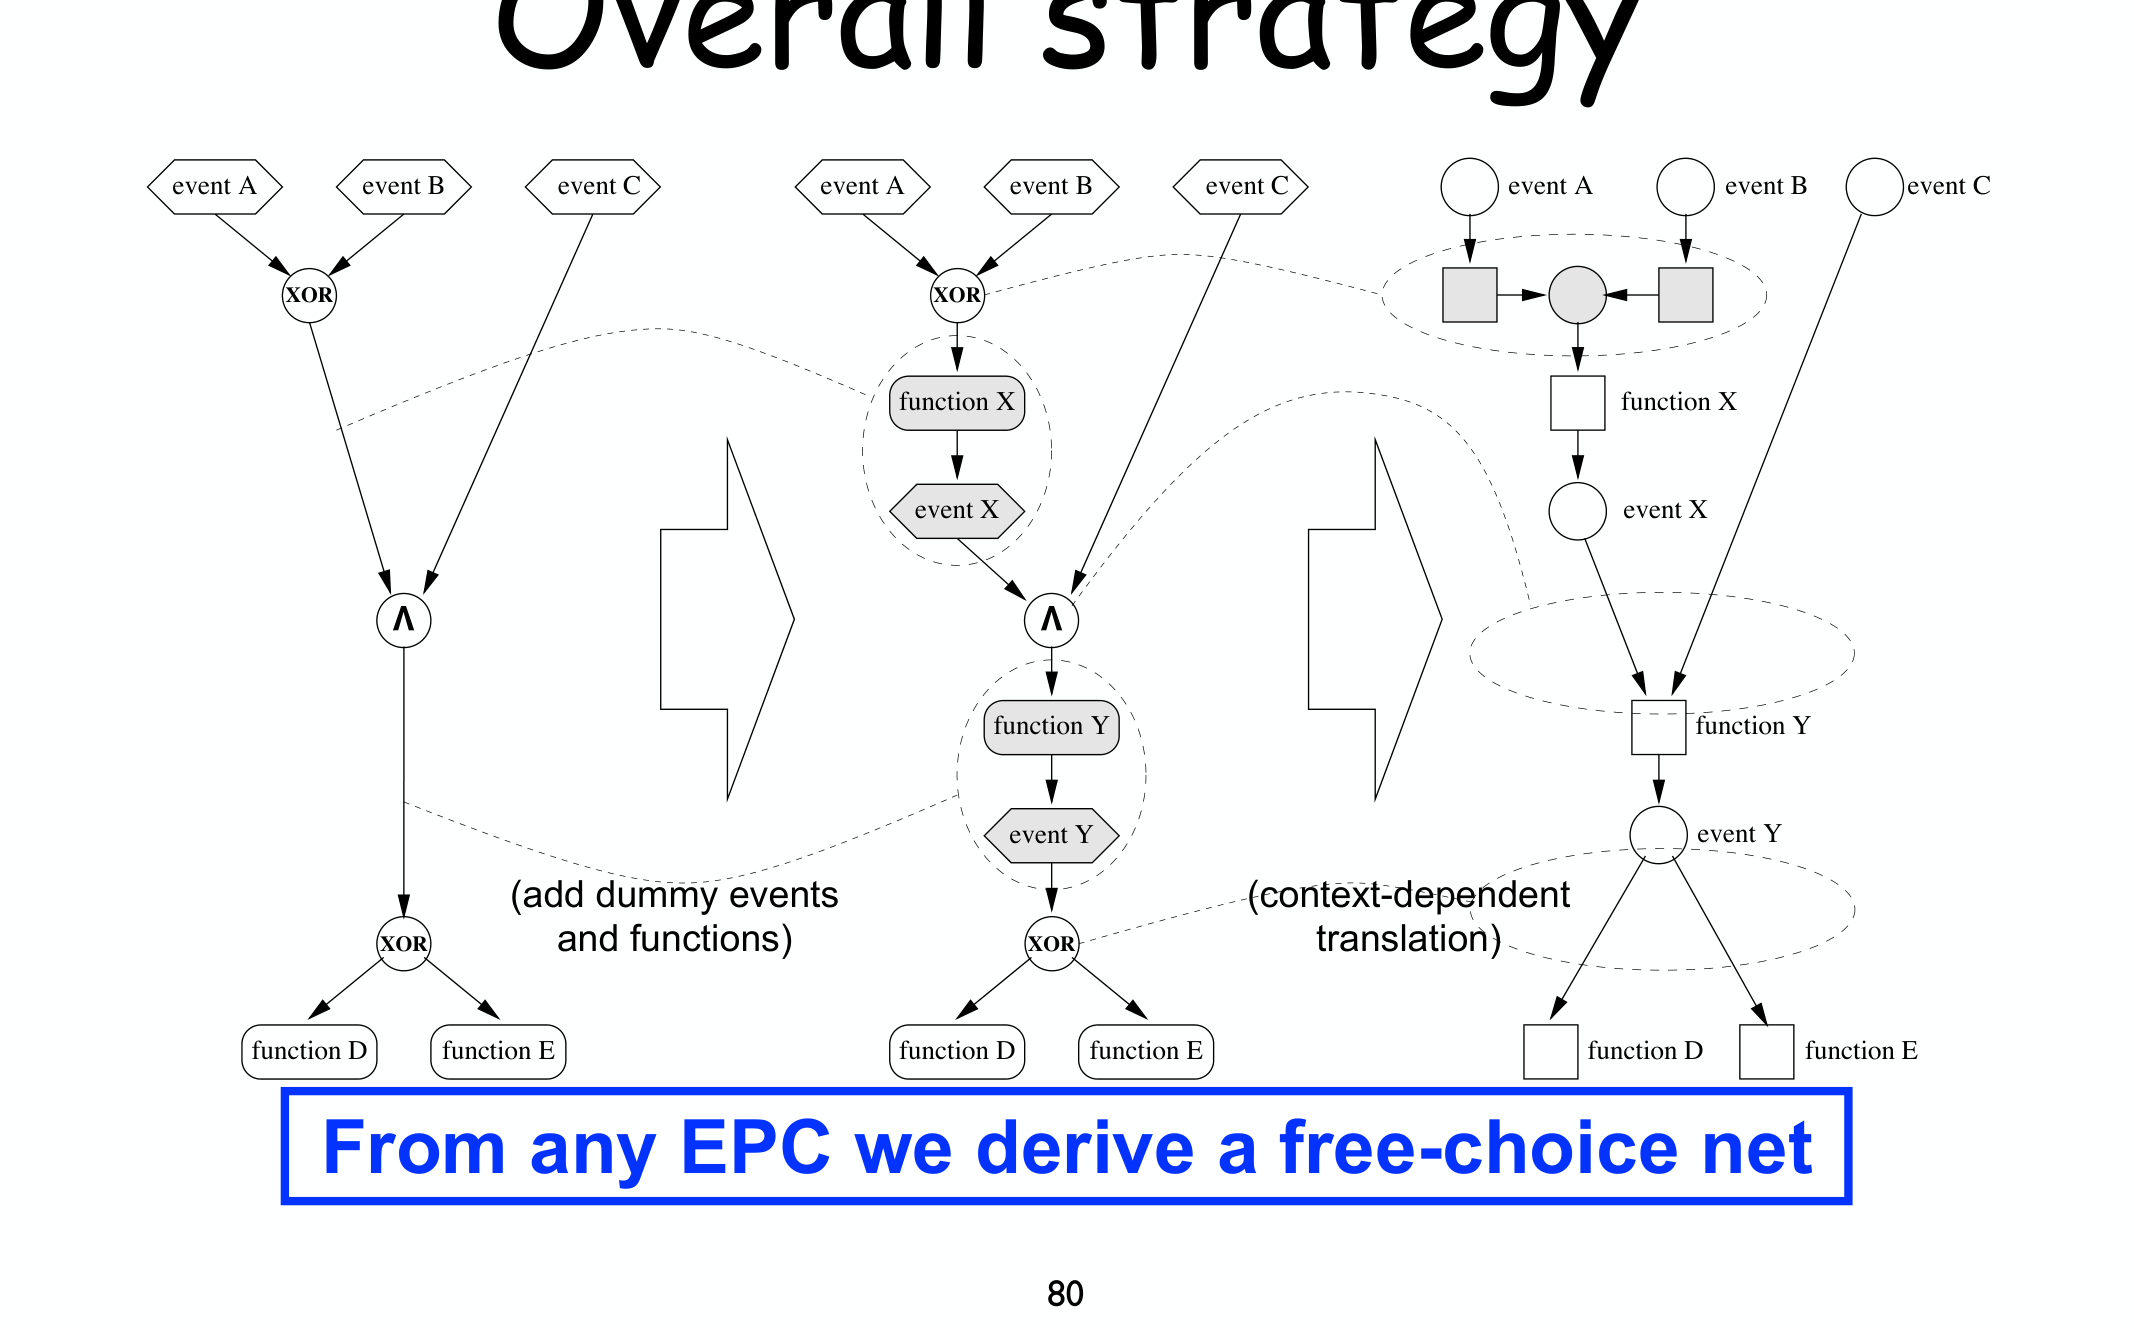
\includegraphics[width=0.74\linewidth,height=0.34\textheight,keepaspectratio]{images/16a-epc-analysis_p80_overall-freechoice.png}
\caption{La strategia complessiva del secondo approccio: dall'EPC (con dummy aggiunti) a un \textbf{free-choice net} tramite traduzione dipendente dal contesto.}
\end{figure}

Il limite resta: se l'EPC contiene OR "essenziali", non si può semplificare senza cambiarne il significato. E anche un EPC semplificato può risultare \textbf{non sound} — ma almeno ora l'analisi è affidabile e trattabile.

\section{\texorpdfstring{Terzo approccio: EPC decorati}{Terzo approccio: EPC decorati}}

Il terzo approccio (Rittgen) è il più potente: si applica a \textbf{qualsiasi} EPC, a patto che il progettista aggiunga delle \textbf{informazioni} (decorazioni) che risolvano le ambiguità. Due requisiti:

\begin{boxdefinition}{Decorated EPC}
\begin{itemize}
\item ogni \textbf{(X)OR join} è \textbf{abbinato a uno split corrispondente} (dello stesso tipo o compatibile) — l'implicit start split conta come match valido;
\item ogni \textbf{OR join} è \textbf{decorato con una policy}, che dice come comportarsi.
\end{itemize}
\end{boxdefinition}

Il senso delle decorazioni è chiarire \emph{quando} una join deve procedere. Il caso pulito è quando la join ha uno \textbf{split corrispondente}: la join sa quanti rami aspettarsi. Quando invece non c'è corrispondenza diretta, serve una policy esplicita.

\begin{boxdefinition}{Le policy dell'OR join}
\begin{itemize}
\item \textbf{wfa — wait-for-all}: aspetta il completamento di \emph{tutti} i cammini attivati. È la semantica naturale quando c'è uno split corrispondente; funziona bene con qualsiasi split.
\item \textbf{et — every-time}: attiva il ramo in uscita a \emph{ogni} input che arriva (possono comparire più token nel target). Adatta a uno split XOR corrispondente.
\item \textbf{fc — first-come}: aspetta il \emph{primo} input e ignora il secondo (possono restare token pendenti). Adatta a uno split XOR corrispondente.
\end{itemize}
\end{boxdefinition}

Per lo \textbf{XOR join} l'assunzione è più rigida: deve \textbf{sempre} avere uno split corrispondente. Nessuna policy (wfa/et/fc) è compatibile con l'esclusività dello XOR — un token da un ramo si può accettare solo se si è certi che dall'altro ramo non ne arriverà mai un secondo, e questa certezza la dà solo lo split corrispondente.

A livello di traduzione, le join decorate diventano frammenti di net specifici (in \textbf{dummy style}, con dummy transition/place dove serve). Anche qui, tuttavia, un EPC decorato può risultare \textbf{non sound}: la decorazione rende l'analisi \emph{accurata}, non garantisce la correttezza.

\section{\texorpdfstring{Il messaggio finale}{Il messaggio finale}}

Nessuno dei tre approcci è "la" soluzione: ciascuno paga un prezzo diverso. È il classico trade-off fra libertà del linguaggio e possibilità di analisi.

\begin{boxabstract}{EPC: pros and cons}
\begin{itemize}
\item Lasci \textbf{libertà completa} (1° approccio) $\rightarrow$ la maggior parte dei diagrammi \textbf{non sarà sound}.
\item \textbf{Vincoli} la sintassi (2° approccio) $\rightarrow$ ma alle persone piace la flessibilità e \textbf{ignorano le linee guida}.
\item Chiedi \textbf{decorazioni} (3° approccio) $\rightarrow$ ma le persone sono pigre o \textbf{fraintendono le policy}.
\end{itemize}
\end{boxabstract}

La lezione mostra così, con un caso reale, che dare semantica formale a un linguaggio informale è tutt'altro che gratuito: l'ambiguità che rende gli EPC comodi da disegnare è la stessa che ne rende difficile la verifica. Nella prossima lezione applichiamo lo stesso spirito d'analisi al BPMN. $\rightarrow$ \hyperref[ch:16b]{16b — BPMN Analysis}